\graphicspath{{\subfix{../images/}}}
%-------------------------------------------
%	Chapter 2: LHC and ATLAS
%-------------------------------------------
\doublespacing

%-------------------------------------------
%	Chapter 2: LHC and ATLAS
%-------------------------------------------
\chapter{Theoretical and Experimental Framework}
\label{chapter-2}

All experiments in high energy physics are guided by the fundamental questions, what the building blocks of matter are and which rules their interactions describe. The Standard Model (SM) of particle physics is the current view of the microscopic world. The experiments currently constructed (and undergoing construction) are expected to probe into its theory and very likely hints on the physics beyond. Since the completion of its construction in 2008, the \ac{LHC} \cite{Evans:2008zzb} at CERN has extended the frontiers of particle physics through its unprecedented energy and luminosity. Located on the Swiss-French border, the \ac{LHC} is the world’s largest particle accelerator. It is designed to accelerate protons around a 27 km ring until they are travelling just 3 ms$^{-1}$ slower than the speed of light, at which point they are made to collide. The protons travel round the ring 11,000 times per second in two concentric beams, which are guided by superconducting magnets, cooled using liquid helium to \num{-271.3} \si{\degree}C (1.9 K). The beams are made to cross at four locations so that collisions between protons can take place. Around these collision points four specialised detectors, ALICE \cite{AliceCollaboration_2008}, CMS \cite{CMS-TDR-08-001}, LHCb \cite{LHCbCollaboration_2008} and ATLAS \cite{PERF-2007-01}, are located to capture information. In this chapter, an introduction to the theoretical framework, including the SM, is given in Section \ref{theo-framework}. A brief overview of the \ac{LHC} is provided in Section \ref{the-lhc}. The ATLAS experiment is presented in Section \ref{atlas-section}. Finally, the future of the \ac{LHC} program is presented in Section \ref{hi-lumi}, with a focus on the motivation and challenges that the  \ac{HL-LHC} phase will bring.

\section{Theoretical Framework}
\label{theo-framework}
This section presents a short introduction into the SM and is included for a more complete picture of the LHC by sketching the physics searches for which it has been designed. A full survey of the presented topics is not intended and the reader is encouraged to search among the available literature for further details.


\subsection{The Standard Model of Particle Physics}
The SM of particle physics \cite{SM-bkg, PhysRevLett.19.1264, GLASHOW1961579} is the theory describing all known elementary particles and their interactions via three of the four fundamental forces. Developed by merging the theories of quantum mechanics and relativity in the second half of the 20th century, the SM’s position today is at the centre of our understanding of the nature of the Universe and is firmly established by an unparalleled level of agreement between the model’s predictions and experimental results \cite{Morel2020-kf}. The SM comprises the unified theory of Quantum Chromodynamics (QCD) and the electro-weak theory; both belong to the group of Quantum Field Theories (QFT).

The SM consists of the fundamental particles that make up all matter \cite{Povh:1995mua}. The building blocks of stable matter are fermions with half-integer spin, following the Fermi-Dirac statistics. In 1928, Dirac deduced the existence of antiparticles when he tried to generalize the Schr\"{o}dinger wavefunction to relativistic quantum mechanics for spin-$\dfrac{1}{2}$ particles. Negative-energy solutions automatically arise in the extension, which he interpreted as "holes" to the vacuum. Anti-particles therefore have the same mass and identical properties as their related particles, but their signs of electric charge and other quantum numbers are reversed. 

Figure \ref{fig: sm-infographic} presents an info-graphic of the SM particles. The fermions in the SM can be divided into three generations, where each generation comprises a double of quarks and a doublet of leptons. The quarks are subdivided into a family of up-type quarks comprising of electric charge +2/3 (up $u$, charm $c$ and top $t$) and down-type quarks comprising of electric charge -1/3 (down $d$, strange $s$ and bottom $b$). The leptons are subdivided into a family of electric charge -1 (electron $e$, muon $\mu$ and tau $\tau$) and a related electrically neutral neutrino (electron-neutrino $\nu_e$, muon-neutrino $\nu_{\mu}$ and tau-neutrino $\nu_{\tau}$). The families are identical copies in their basic properties beside their mass.


\begin{figure}[htb!]
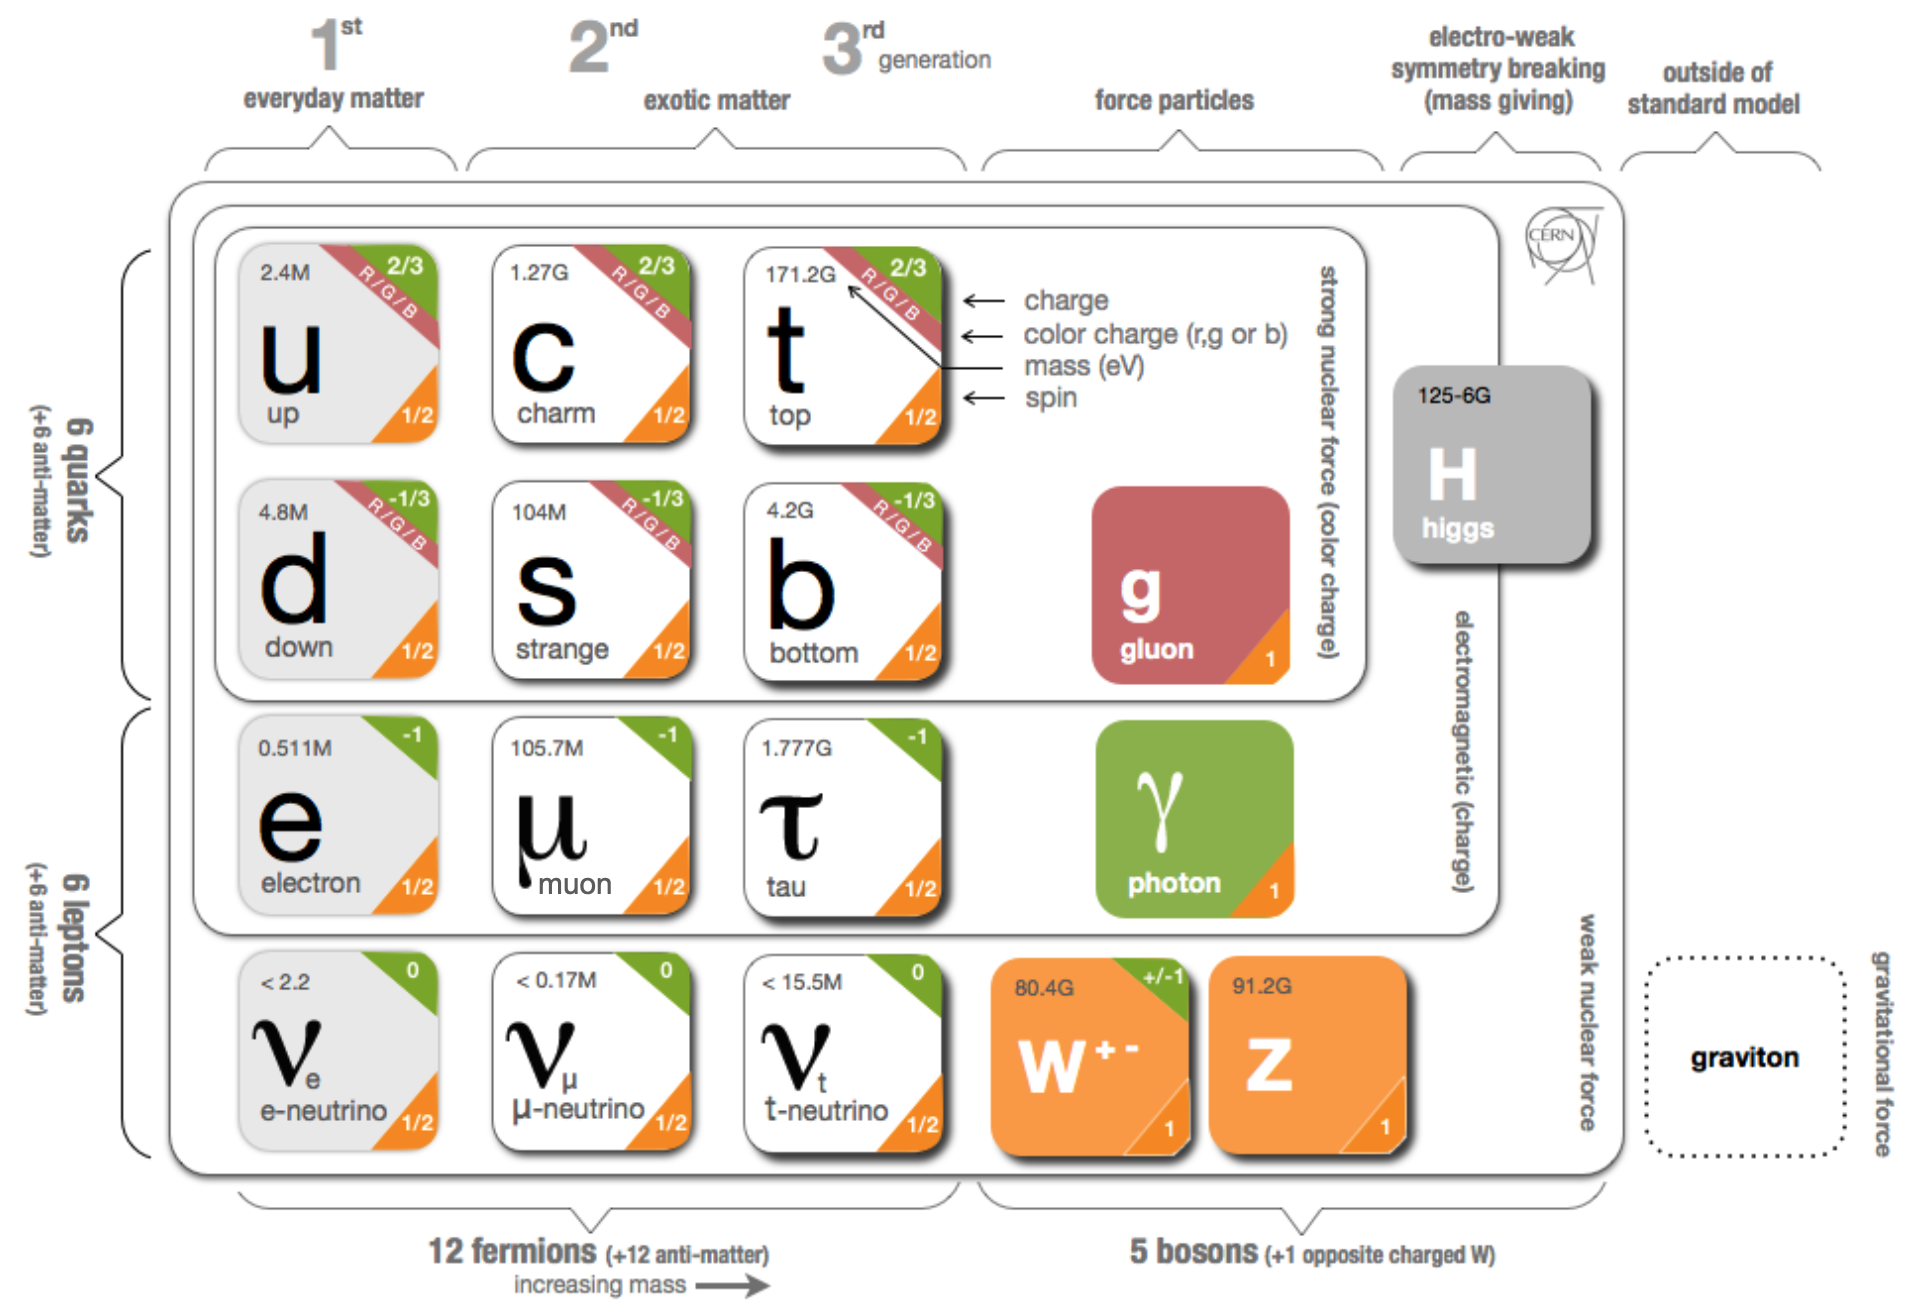
\includegraphics[width=\textwidth]{images/2-LHC-ATLAS/SM-infographic.png}
\caption{Info-graphic of the Standard Model particles \cite{david_galbraith_ux_2012}. The mediators of the different interactions are denoted by force particles. It can be seen that neutrinos interact only through the weak force, while charged leptons interact via the electromagnetic and weak forces, and quarks can interact through all three of the fundamental forces in the Standard Model.}
\label{fig: sm-infographic}
\end{figure}

The leptons are sensitive to the weak and electromagnetic interactions. The neutrinos weakly interact with matter; they oscillate between generations due to the non-zero neutrino mass and neutrino mixing \cite{Bilenky_1999}. The quarks are sensitive to the three interactions; strong, electromagnetic and weak. 

Central to QFT is the Lagrangian density which describes the kinematics and dynamics of a field, as well as observations of conserved quantities linking to symmetries. A full derivation of the Lagrangian formalism used in particle physics can be found in Ref \cite{gauge-theories}. A basic principle of each QFT are gauge symmetries \cite{bailin1993introduction}. Using the principle of local gauge theories, one can derive the existence of bosons from first principles. The bosons belong to the gauge fields needed to obtain a consistent theory with interactions between the fermions. Bosons have integer spin, following the Bose-Einstein statistics, that transmit interactions (force carriers), or the constituents of radiation. The force carrier of the electromagnetic interaction is the photon, $\gamma$. The weak interaction has three massive gauge mediators called $Z^{0}$ and $W^{\pm}$ bosons with a short range of interaction. The strong interaction is mediated by eight massless gluons, which carry color\footnote{The word \textbf{colour} in QCD is an arbitrarily chosen terminology, and not related to our common conception of colour in visible light.} charge. 

As the gluons are themselves coloured, if one attempts to separate two quarks, the energy within the gluon field increases until it becomes energetically favourable for a new quark/anti-quark pair to form in the the vacuum than to allow the quarks to separate further. As a result of this, when quarks are produced in particle detector experiments, clustered jets of colour-neutral particles (hadrons) are observed, known as \textit{hadronization}. The hadrons are a result of this confinement of quarks and gluons, and they are bound in combinations called hadrons, where three bounded quarks are named “baryons” (e.g. protons and neutrons) and quark-antiquark pairs are named “mesons” (e.g. $\pi$, $K$ and $B$).

Unifying the theory of the strong, weak and electromagnetic fundamental forces, as well as the fundamental particles of matter, the SM does not describe gravity and is therefore not a complete theory of the fundamental interactions.





\subsection{The Higgs Sector}

The Higgs boson is the latest SM particle found, first theorised in the 1960s \cite{PhysRevLett.13.321, PhysRevLett.13.508, PhysRevLett.13.585}. The Higgs boson is a remnant of the Spontaneous Symmetry Breaking (SSB) mechanism of the electro-weak interaction that provides a mass to the SM particles \cite{doi:10.1098/rsta.2014.0033}. The Higgs particle, a spin-0 boson, is linked to the Higgs mechanism. In this theory, it is proposed that the entirety of space is permeated by the Higgs field. A particle that interacts with the Higgs field acquires its mass from moving through it, where the mediating particle is the Higgs boson. In addition, the Higgs boson can couple to any other particle which has mass, including itself (self-coupling). Further information on the Higgs mechanism can be found in \cite{Bednyakov_2008}. 

The Higgs boson is a short lived particle (approximately $10^{-22})$ seconds), so it cannot be detected directly. However, it can decay to different types of particles which can be detected. It was eventually observed by the ATLAS and CMS experiments at the LHC in 2012 \cite{higgs-20121, higgs-201230}. After its discovery, further ongoing work has been carried out performing detailed measurements of its mass and interactions with other particles. The main production and decay channels for the Higgs boson are shown in Figure \ref{fig: higgs}.

\begin{figure}[htb!]
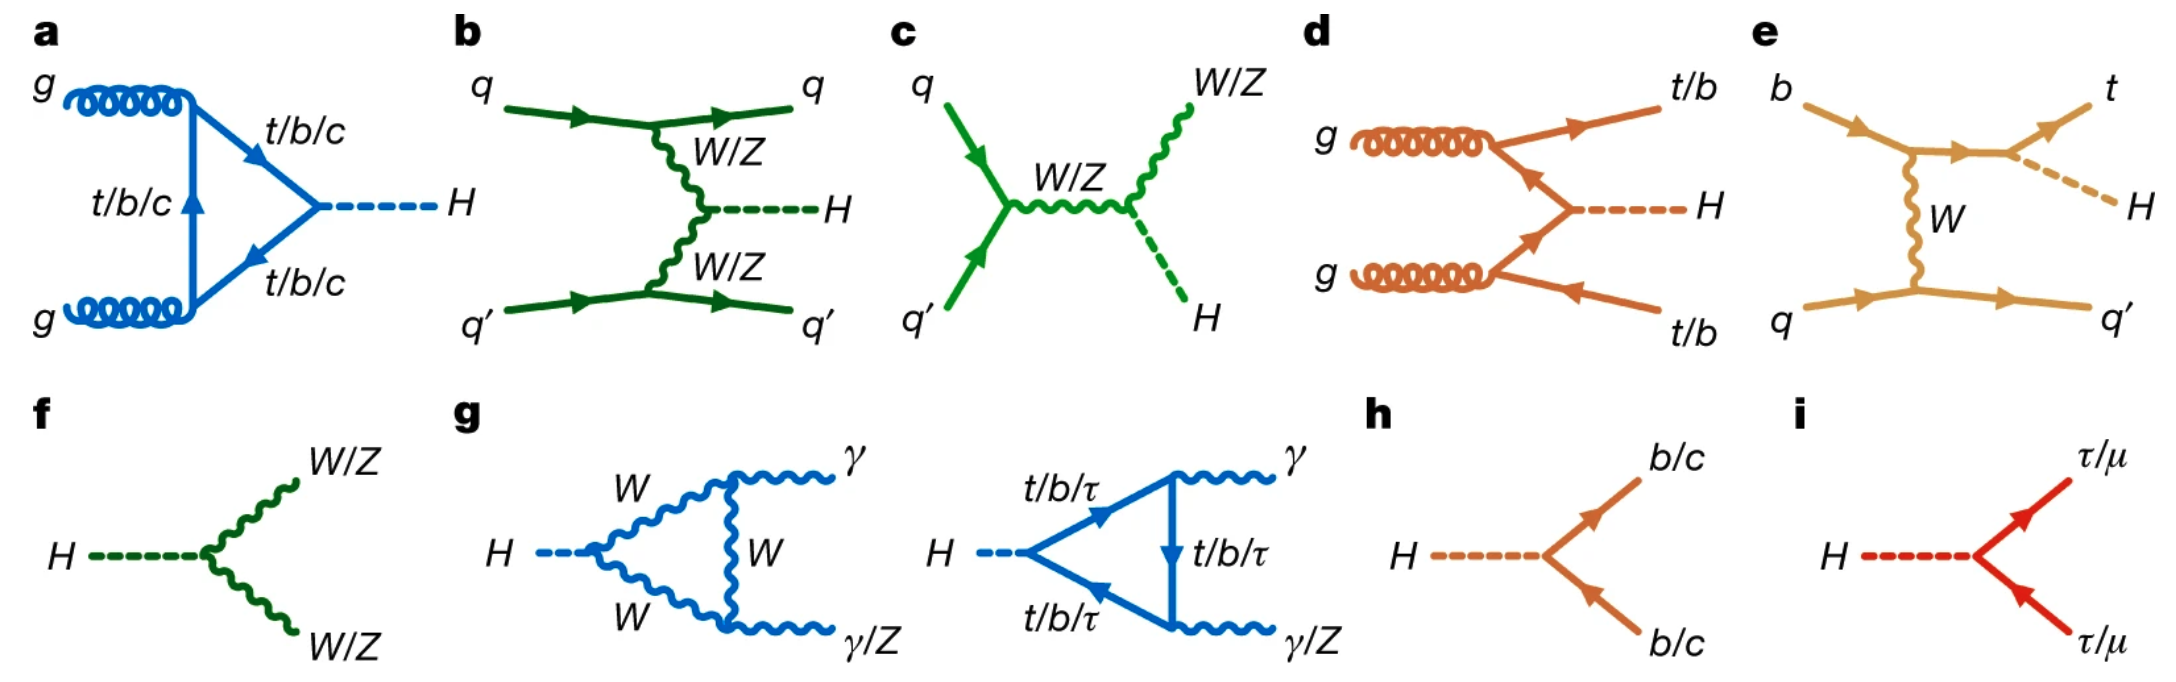
\includegraphics[width=\textwidth]{images/2-LHC-ATLAS/higgs.png}
\caption{Examples of Feynman diagrams for Higgs boson production and decays \cite{ATLAS:2022vkf}. The Higgs boson is produced via (a) gluon–gluon fusion, (b) vector-boson fusion (VBF), (c) VBF and associated production with vector bosons, (d) top or quark pairs, or (e) a single top quark. The Higgs boson decays into (f) a pair of vector bosons,(g)  a pair of photons or a boson and a photon, (h) a pair of quarks, and (i) a pair of charged leptons.}
\label{fig: higgs}
\end{figure}






\section{The Large Hadron Collider}
\label{the-lhc}
The \ac{LHC} is operated in multi-year runs during which beams of protons travelling in opposite directions are circulated and collide. Between runs there are periods of shutdown, while the accelerator and detector machinery is maintained and upgraded. Run 1 began in 2010 when the \ac{LHC} collided proton bunches, each containing more than $10^{11}$ particles, 20 million times per second, providing 7 TeV proton-proton collisions at instantaneous luminosities of up to 2.1 $\times$ 10$^{32}$ cm$^{−2}$s$^{−1}$.

The centre-of-mass energy was increased to 8 TeV towards the end of Run 1 in 2012. Run-2, which spanned 2015–2018, further increased the proton-proton collision energy to 13 TeV. During Run-2, the bunch spacing was reduced, leading to a collision rate of 40 MHz. Over the course of Run-2, a total usable integrated luminosity of 139 fb$^{−1}$ was recorded. 2022 marked the beginning of Run-3, which, with a higher center of mass energy of 13.6 TeV and peak luminosity at 2 $\times$ 10$^{34}$ cm$^{−2}$s$^{−1}$, is expected to culminate in the approximate tripling of the dataset size. In addition, the number of proton-proton (pp) collisions per bunch crossing, referred to collectively as pile-up, is expected to be $\langle \mu \rangle$ = 60-65 at the end of Run-3. A summary of key information about each run is listed in Table \ref{tab:lhc-runs}.

\begin{table}[!htbp]
  \footnotesize\centering
  \setlength{\tabcolsep}{0.5em} % for the horizontal padding
  \begin{tabular}{cc|cccc}
      \toprule
      \textbf{Period} & \textbf{Year} & $\sqrt{s}$ [TeV] 
      & $\langle \mu \rangle$ & \textbf{Bunch spacing} [ns] & \textbf{Luminosity} [cm$^{−2}$s$^{−1}$] \\
      \hline
      Run-1 & 2010--2012 & \SIrange[range-phrase=--,range-units=single,range-exponents=combine]{7}{8}{} & 18 & 50 & $8 \times 10^{33}$ \\
      Run-2 & 2015--2018 & \SI{13  }{} & 34 & 25 & $1\textnormal{--}2 \times 10^{34}$ \\
      Run-3 & 2022--2025 & \SI{13.6}{} & 60-65 & 25 & $2 \times 10^{34}$ \\
      \bottomrule
  \end{tabular}
  \caption{
    Overview of the different \ac{LHC} runs \cite{atlas-lumi-run1,atlas-lumi-run2}.
    The average number of interactions per bunch-crossing is denoted as $\langle \mu \rangle$, and is here averaged over the entire run. Numbers for Run-3 are preliminary and are only provided to give an indication of expected performance.
    % run 1 run 2 trigger https://cds.cern.ch/record/2058218/
    %  2-3 × 1034 cm−2 s−1 and an average pile-up of ~80 collisions/bunch-crossing
    % https://cds.cern.ch/record/2732959/files/LHCP2020_094.pdf
  }
  \label{tab:lhc-runs}
\end{table}

An overview of the accelerator complex at CERN is shown in Figure \ref{fig: accelerator-complex}. The \ac{LHC} is at the final stage of a chain of accelerators which incrementally step-up the energy of incoming protons. The first accelerator is Linac4, a linear accelerator which accelerates hydrogen atoms to an energy of 160 MeV. Upon leaving Linac4, the hydrogen atoms are stripped of their electrons and the resulting protons are fed into the Proton Synchrotron Booster (PSB), which increases the energy of the protons to 2 GeV. The protons leaving the PSB are passed to the Proton Synchrotron (PS), which increases the energy to 26 GeV, and then from the PS to the Super Proton Synchrotron (SPS), which further increases the energy to 450 GeV. Finally, the proton beams are injected in the \ac{LHC} where they are accelerated to their final energy of 6.5 TeV for Run 2.

\begin{figure}[htb!]
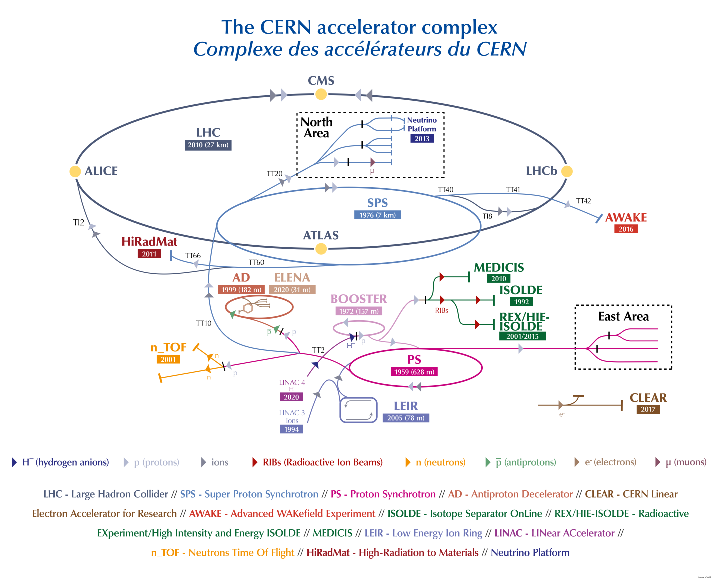
\includegraphics[width=\textwidth]{images/2-LHC-ATLAS/accelerator_complex.pdf}
\caption{An overview of the CERN accelerator complex \cite{CERN:2012:accelerators}. The \ac{LHC} is fed by a series of accelerators starting with Linac4. Next are the Proton Synchrotron Booster, the Proton Synchrotron, and finally the Super Proton Synchrotron which injects protons into the \ac{LHC}.}
\label{fig: accelerator-complex}
\end{figure}



%-------------------------------------------
%	Chapter 2: ATLAS
%-------------------------------------------
\section{The ATLAS Experiment}
\label{atlas-section}

\subsection{The ATLAS Detector}
The ATLAS detector is one of two general-purpose detectors in operation at the \ac{LHC} \cite{PERF-2007-01}. The experiment aims to make Standard Model (SM) precision measurements and test Beyond Standard Model (BSM) theories. In total, the detector is a 44 m long cylinder with a diameter of 25 m and weighs over 7000 tonnes, shown in Figure \ref{fig: atlas-detector}. The detector’s geometry is cylindrical consisting of a central barrel and two end-caps to ensure forward physics coverage and hermeticity. The ATLAS detector comprises of specialised sub-detectors, orientated coaxially around the nominal interaction point at the centre of the detector. 

\begin{figure}[htb!]
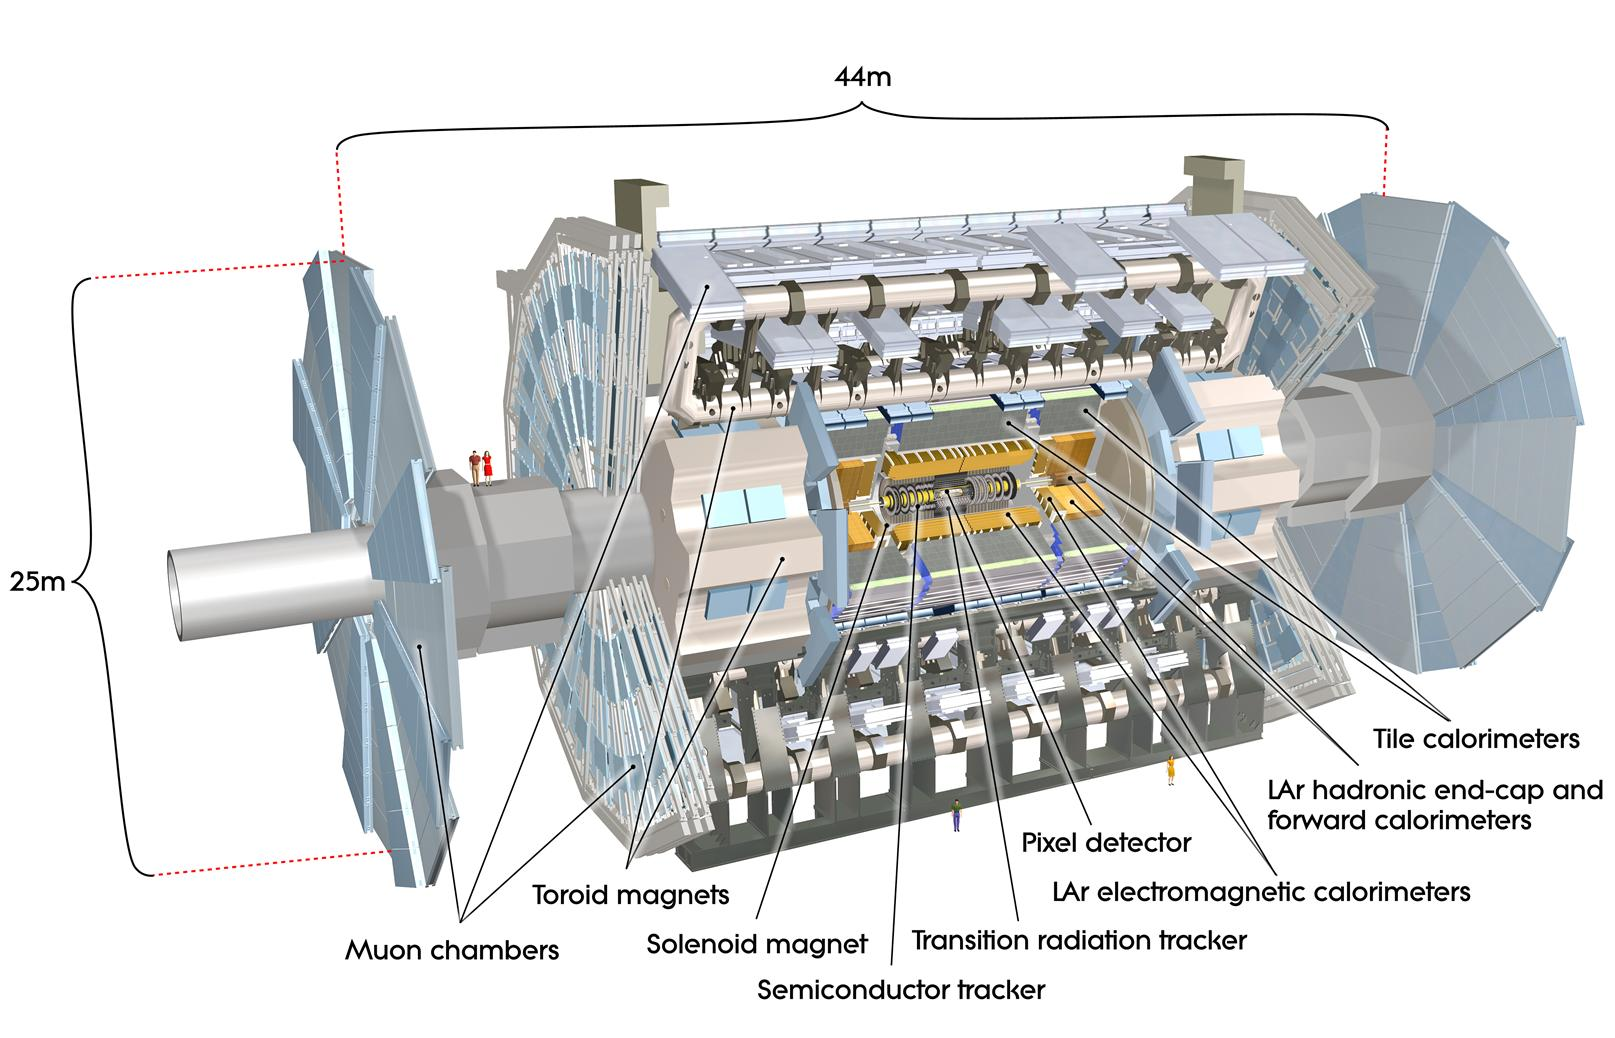
\includegraphics[width=\textwidth]{images/2-LHC-ATLAS/atlas_detector.jpg}
\caption{A 3D model of the entire ATLAS detector \cite{Jon-And:1237407}. Cutouts to the centre of the detector reveal the different sub-detectors which are arranged in concentric layers around the nominal interaction point.}
\label{fig: atlas-detector}
\end{figure}

In order of increasing radial distance, the ATLAS sub-detectors include the Inner Detector (ID) described in Section \ref{inner-detector}, the electromagnetic and hadronic calorimeters, and the outermost muon spectrometer. 

More comprehensive descriptions of the calorimeters and muon spectrometer can be found in the Technical Design Report for the ATLAS detector \cite{inner-detector-TDR}. Since the work in this thesis pertains to tracking, particular attention is given to the Inner Detector (ID) which houses the tracking systems of the ATLAS detector. In Section \ref{coordinate-system}, the coordinate system used at ATLAS and definitions for frequently occurring quantities are also provided.



%-------------------------------------------
%	Chapter 2: Coordinate system
%-------------------------------------------
\subsection{Coordinate System and Collider Definitions}
\label{coordinate-system}

%% based on https://twiki.cern.ch/twiki/bin/view/AtlasProtected/PubComCommonText

\subsubsection{The ATLAS Coordinate System}

The origin of the coordinate system used by ATLAS is the nominal interaction point in the centre of the detector. As shown in Figure \ref{fig:atlas-coord-system}, the z-axis points along the direction of the beam pipe, while the x-axis points from the interaction point to the centre of the \ac{LHC} ring, and the y-axis points upwards.
The transverse plane lies in $x$-$y$ while the longitudinal direction lies along the z-axis. A cylindrical coordinate system with coordinates ($r$,$\phi$) is used in the transverse plane, where $r$ is the radius from the origin and $\phi$ is the azimuthal angle around the z-axis.

\begin{figure}[!htbp]
  \centering
  % Author: Izaak Neutelings (June 2017)
% taken from https://tex.stackexchange.com/questions/159445/draw-in-cylindrical-and-spherical-coordinates
% Licensed under CC Attribution-Share Alike 4.0 International  https://creativecommons.org/licenses/by-sa/4.0/
% Original source https://wiki.physik.uzh.ch/cms/latex:example_spherical_coordinates
% Modifications by Giles Strong (March 2020):
% 1. Removal of some header code
% 2. Changing theta to eta
% 3. Addition of mountains
% 4. Changed "\draw[dashed,red] (O)  -- (Pxy);" to "\draw[->] (O)  -- (Pxy) node[right] {$p_t$};"
% Modifications by Giles Strong (April 2020):
% 1. Removal of Jura mountains
% 2. Rotated to be in terms of ATLAS coordinate system
% 3. Resized labels for the detectors

\tikzset{>=latex} % for LaTeX arrow head

\tdplotsetmaincoords{76}{45} % to reset previous setting 75 50
    \begin{tikzpicture}[scale=4.8,tdplot_main_coords,rotate around x=90]
    
    % variables
    \def\rvec{1.2}
    \def\thetavec{40}
    \def\phivec{70}
    \def\R{1.1}
    \def\w{0.3}
    
    % axes
    \coordinate (O) at (0,0,0);
    \draw[thick,->] (0,0,0) -- (1,0,0) node[below left]{$x$};
    \draw[thick,->] (0,0,0) -- (0,1,0) node[below right]{$y$};
    \draw[thick,->] (0,0,0) -- (0,0,1) node[below right]{$z$};
    \tdplotsetcoord{P}{\rvec}{\thetavec}{\phivec}
    
    % vectors
    \draw[->,red] (O) -- (P) node[above left] {$\vec{p}$};
    \draw[->] (O)  -- (Pxy) node[right] {$p_T$};
    \draw[dashed,red] (P)  -- (Pxy);
    \draw[dashed,red] (Py) -- (Pxy);
    
    % circle - LHC
    \tdplotdrawarc[thick,rotate around x=90,black!70!blue]{(\R,0,0)}{\R}{0}{360}{}{}
    
    % compass - the line between CMS and ATLAS has a ~12° declination (http://googlecompass.com)
    %\begin{scope}[shift={(1.1*\R,0,1.65*\R)},rotate around y=12]
    %    \draw[<->,black!50] (-\w,0,0) -- (\w,0,0);
    %    \draw[<->,black!50] (0,0,-\w) -- (0,0,\w);
    %    \node[below right,black!50,scale=0.6] at (\w,0,0) {N};
    %\end{scope}
    
    % nodes
    \node[right] at (\R,0,0) {LHC};
    \fill[radius=0.8pt,black!20!red]
        (O) circle node[left=4pt,below=5pt] {ATLAS};
    \draw[thick] (0.02,0,0) -- (0.5,0,0); % partially overdraw x-axis and CMS point
    \fill[radius=0.8pt,black!20!blue]
        (2*\R,0,0) circle
        node[right=4pt,below=2pt,scale=0.7] {CMS};
    \fill[radius=0.8pt,black!10!orange]
        ({-\R*sqrt(2)/2+\R},0,{-\R*sqrt(2)/2}) circle % 45 degrees from ATLAS
        node[left=2pt,below=2pt,scale=0.7] {ALICE};
    \fill[radius=0.8pt,black!60!green]
        ({-\R*sqrt(2)/2+\R},0,{\R*sqrt(2)/2}) circle % 45 degrees from ATLAS
        node[below=6pt,right=3pt,scale=0.7,anchor=north east] {LHCb};
    
    % arcs
    \tdplotdrawarc[->]{(O)}{0.2}{0}{\phivec}
        {above=2pt,right=-1pt,anchor=mid west}{$\phi$}
    \tdplotdrawarc[->,rotate around z=\phivec-90,rotate around y=-90]{(0,0,0)}{0.5}{0}{\thetavec}
        {anchor=mid east}{$\eta$}
\end{tikzpicture}
  \caption{
    The coordinate system used at the ATLAS detector, showing the locations of the four main experiments located at various points around the \ac{LHC}. The 3-vector momentum $p_{\text{T}} = (p_x, p_y, p_z)$ is shown by the red arrow. Reproduced from \cite{Strong:2020mge}.
  }
  \label{fig:atlas-coord-system}
\end{figure}

Additionally, the transverse $x$-$y$ plane is often used to describe the kinematics of collisions, where the transverse momentum $p_{\text{T}}$ of an object is the projection of its momentum on the transverse plane, given by Eq \ref{eq:pt}.

%
\begin{equation}\label{eq:pt}
  p_\text{T} = \sqrt{ {p_x}^2 + {p_y}^2 }
\end{equation}



%The pseudorapidity is defined in terms of the polar angle $\theta$ as $\eta = -\ln \tan(\theta/2)$.


\subsubsection{Pseudorapidity}

The pseudorapidity, $\eta$, is a commonly used spatial coordinate describing the polar angle, $\theta$, of a particle's trajectory relative to the beam axis, and is defined as:
%
\begin{equation}\label{eq:pseudorap}
  \eta = - \ln \left[ \tan \left( \frac{\theta}{2} \right) \right] .
\end{equation}
%
The pseudorapidity is a convenient quantity to work with as differences in $\eta$ are invariant under Lorentz boosts. In addition, particle production is constant as a function of $\eta$.


%-------------------------------------------
%	Chapter 2: The Inner Detector
%-------------------------------------------
\subsection{The Inner Detector}
\label{inner-detector}

The ID system provides high-resolution charged particle trajectory tracking in the range $ \lvert \eta \rvert < 2.5$. The ID is immersed in a 2 T axial magnetic field, produced by a superconducting solenoid magnet, which enables the measurement of particle momentum and charge. The ID is made up of several sub-systems shown in Figures \ref{fig:atlas-id-run1} and \ref{fig:atlas-id-run2}. Each sub-system contains specialised hardware and contributes towards a full track reconstruction. 

\begin{figure}[!htbp]
  \centering
  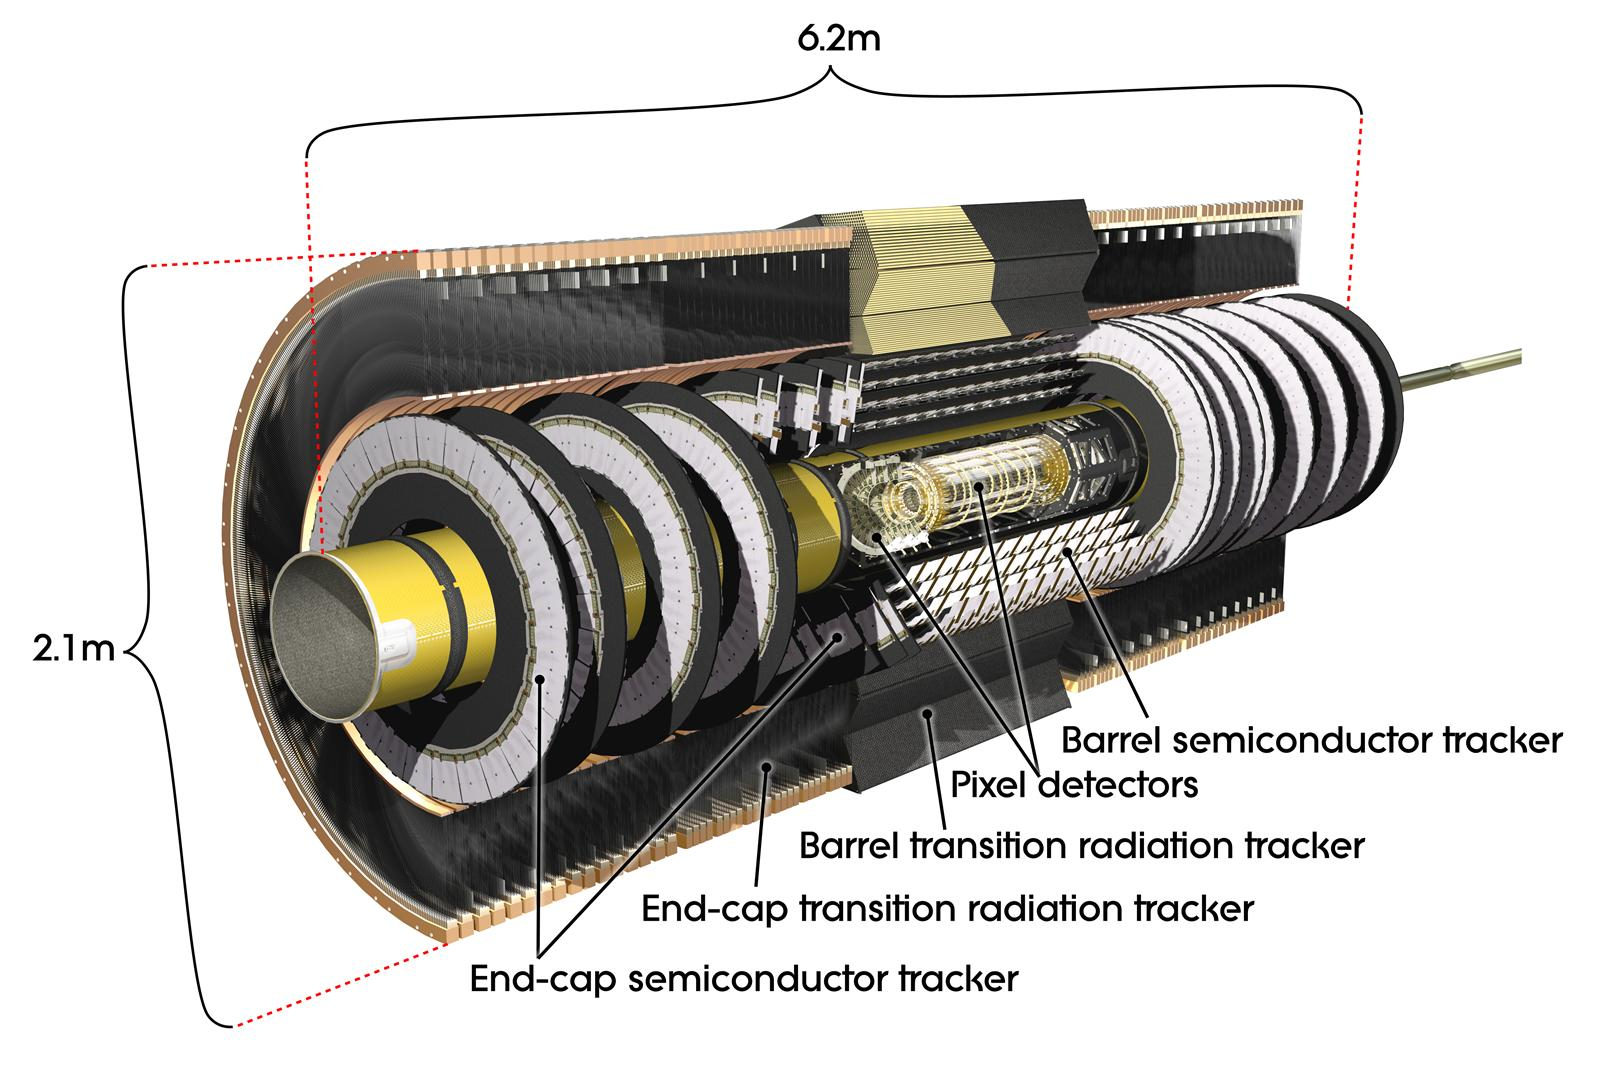
\includegraphics[width=0.85\textwidth]{images/2-LHC-ATLAS/atlas_id.jpg}
  \caption{
    A 3D model of the ATLAS ID, made up of the pixel and semi-conductor tracker sub-detectors, showing the barrel layers and end-cap disks \cite{atlasid}.
  }
  \label{fig:atlas-id-run1}
\end{figure}

\begin{figure}[!htbp]
  \centering
  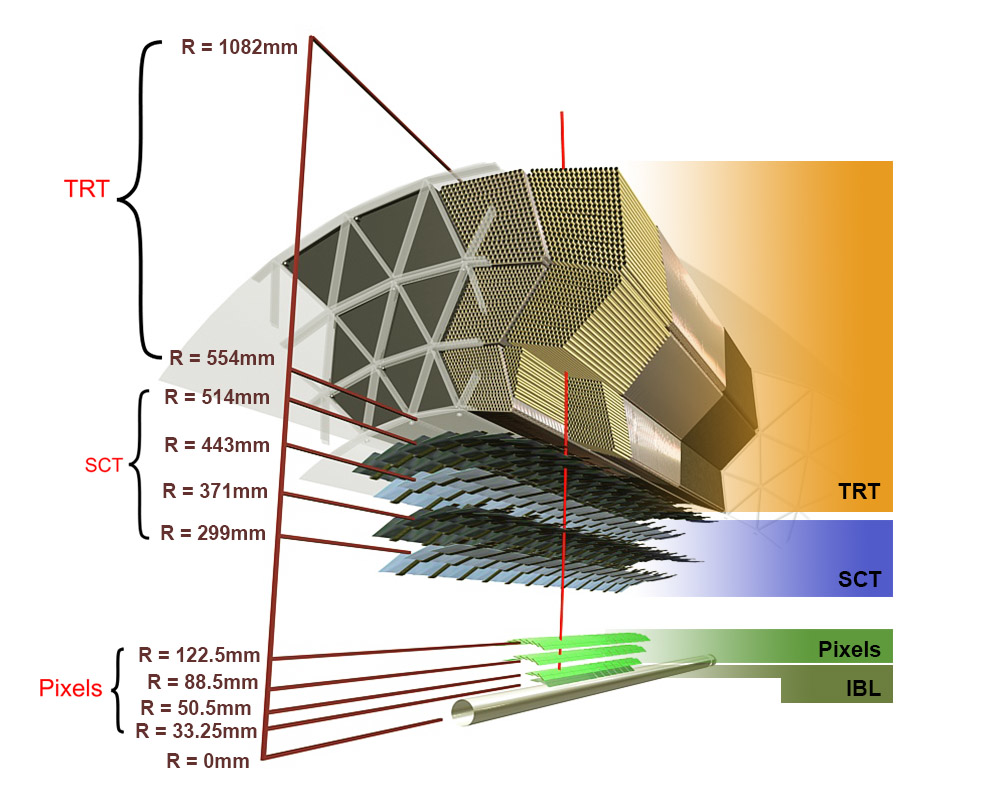
\includegraphics[width=0.85\textwidth]{images/2-LHC-ATLAS/atlas_id_xs.png}
  \caption{
    A cross-sectional view of the ATLAS ID, with the radii of the different barrel layers shown \cite{atlastrackingdocs}.
  }
  \label{fig:atlas-id-run2}
\end{figure}

\subsubsection{Pixel Detector}

The innermost silicon pixel detector \cite{pixel} provides high-granularity measurements covering the interaction region and typically provides four space-point measurements per track. The silicon pixel detector comprises four cylindrical barrels at increasing radii from the beamline, and four end-cap disks on each side. The innermost barrel layer is the Insertable B-layer (IBL), which was installed before Run 2 \cite{ATLAS-TDR-19,PIX-2018-001} and lies approximately just 33 mm from the beam axis. The second-to-innermost layer is often referred to as the B-layer. The pixel detector was initially constructed with 80 million readout channels, with the IBL providing an additional 12 million \cite{ibl}. The specification of the pixel detector determines the impact parameter resolution and the ability to reconstruct primary and secondary vertices. Individual pixels are 50 $\mu$m in the transverse direction (see Section \ref{coordinate-system} for the ATLAS coordinate system) and 400 $\mu$m in the longitudinal $z$ direction (250 $\mu$m for the IBL). Cluster positions have a resolution of approximately 10 $\mu$m in $(r,\phi)$ and 100 $\mu$m in $z$.


\subsubsection{Semi-Conductor Tracker (SCT)}

The pixel detector is followed by the SCT, which is made up of four concentric barrel layers in the central region, and nine disks in each end-cap. Each layer is itself made of a pair of silicon microstrip layers, with a small stereo angle (40 mrad) between the two layers enabling the $z$-coordinate to be measured from a pair of strip measurements. The operation of the silicon sensors is based on the properties of the p-n junction \cite{6773080}. At the junction between the p-type doped silicon and the n-type doped silicon the electrons (holes) diffuse from the n-type (p-type) side and recombine with holes (electrons) on the p-type (n-type) side. The diffusion of the electrons (holes) leaves behind ionised donor (acceptor) atoms and an electric field develops across the junction which inhibits further diffusion until equilibrium is reached. The space charge region formed around the junction is now devoid of mobile charge carriers and is referred to as the depletion region. Applying an external reverse bias voltage to the p-n junction draws electrons (holes) away from the n-type (p-type) side and increases both the depletion region width and the electric field across the junction. Ionising particles traversing the sensor create electron-hole pairs in the depletion region, which are swept to the electrodes by the electric field and induce an electrical current in the external circuitry. In silicon microstrip sensors, like those in the SCT, one (or both) of the electrodes are segmented in order to provide position measurements. The SCT typically provides a further four space-point measurements (eight strip measurements, or hits) per track in the barrel region. See Ref. \cite{inner-detector-TDR} for further information.


\subsubsection{Transition Radiation Tracker (TRT)}

The TRT is a straw-tube tracker which complements the higher-resolution silicon- based tracks by offering a larger number of hits per track and a long lever arm. This aids the accurate measurement of particle momentum and enables radially extended track reconstruction up to $ \lvert \eta \rvert = 2.0$. It is made up of approximately 300,000 drift tubes with a diameter of 4 mm which are filled with an argon/xenon gas mixture. The walls of each tube are electrically charged, and a thin conducting wire runs along the center. When a charged particle traverses a tube, it ionises the gas and the resulting liberated electrons drift along the electric field to the wire, and cascade in the very strong electric field close to the wire, where an associated charge is registered. In the barrel the straws run parallel to the z-axis and therefore the TRT only provides tracking information in $(r, \phi)$. Straws are arranged radially in the end-caps. The resulting two-dimensional space-points have a resolution of approximately 120 $\mu$m. The spaces between the straws are filled with a polymer which encourages the emission of transition radiation, aiding electron identification. Therefore, the TRT combines continuous tracking capabilities with particle identification based on transition radiation (TR).

%Outside of the pixel detector, the SCT measures charged particles at an intermediate distance from the collision point and improves the determination of vertex position and track momentum. The SCT consists of four barrel layers and nine end-cap layers on each side. The outermost section of the ID, the TRT, is used for the identification of charged particles and consists of drift tubes that are filled with a mixture of Xe, CO2 and O2, and contain a central gold-plated tungsten wire. When charged particles traverse the TRT, the gas inside the straws is ionised and the free electrons drift towards the wire and are amplified and then read out. In addition, transition radiation provides information on the particle type that passed through the tracker.





%-------------------------------------------
%	Chapter 2: TDAQ
%-------------------------------------------
\subsection{The Trigger}
The 25 ns bunch spacing used over the course of Run 2 corresponds to a bunch-crossing or event rate of 40 MHz (see Table \ref{tab:lhc-runs}). If the full information for the detector was written out for each event, this would correspond to the generation of 60 TB of data each second. This is more than feasibly possible for the read out from the hardware, the processing and storage of the data. This requires the use of a trigger system which quickly makes a decision about whether or not an event is potentially interesting and should be kept for further analysis. The trigger system comprises two levels which search for signs of electrons, muons, taus, photons and jets, as well as events with large total or missing transverse energy. The hardware-based Level-1 (L1) trigger uses coarse information from the calorimeters and muon spectrometer to accept events at an average rate of 100 kHz approximately 2.5 $\mu$s after the event. After the L1 trigger, the software-based High Level Trigger (HLT) makes use of 40,000 CPU cores to make a final selection on surviving events, using full granularity detector information in approximately 200 ms. The final event read-out rate is approximately 1.2 kHz, corresponding to 1.2 GBs$^{-1}$ of permanent data storage. More information is provided in \cite{TRIG-2016-01}.

\begin{figure}[htb!]
    \centering
    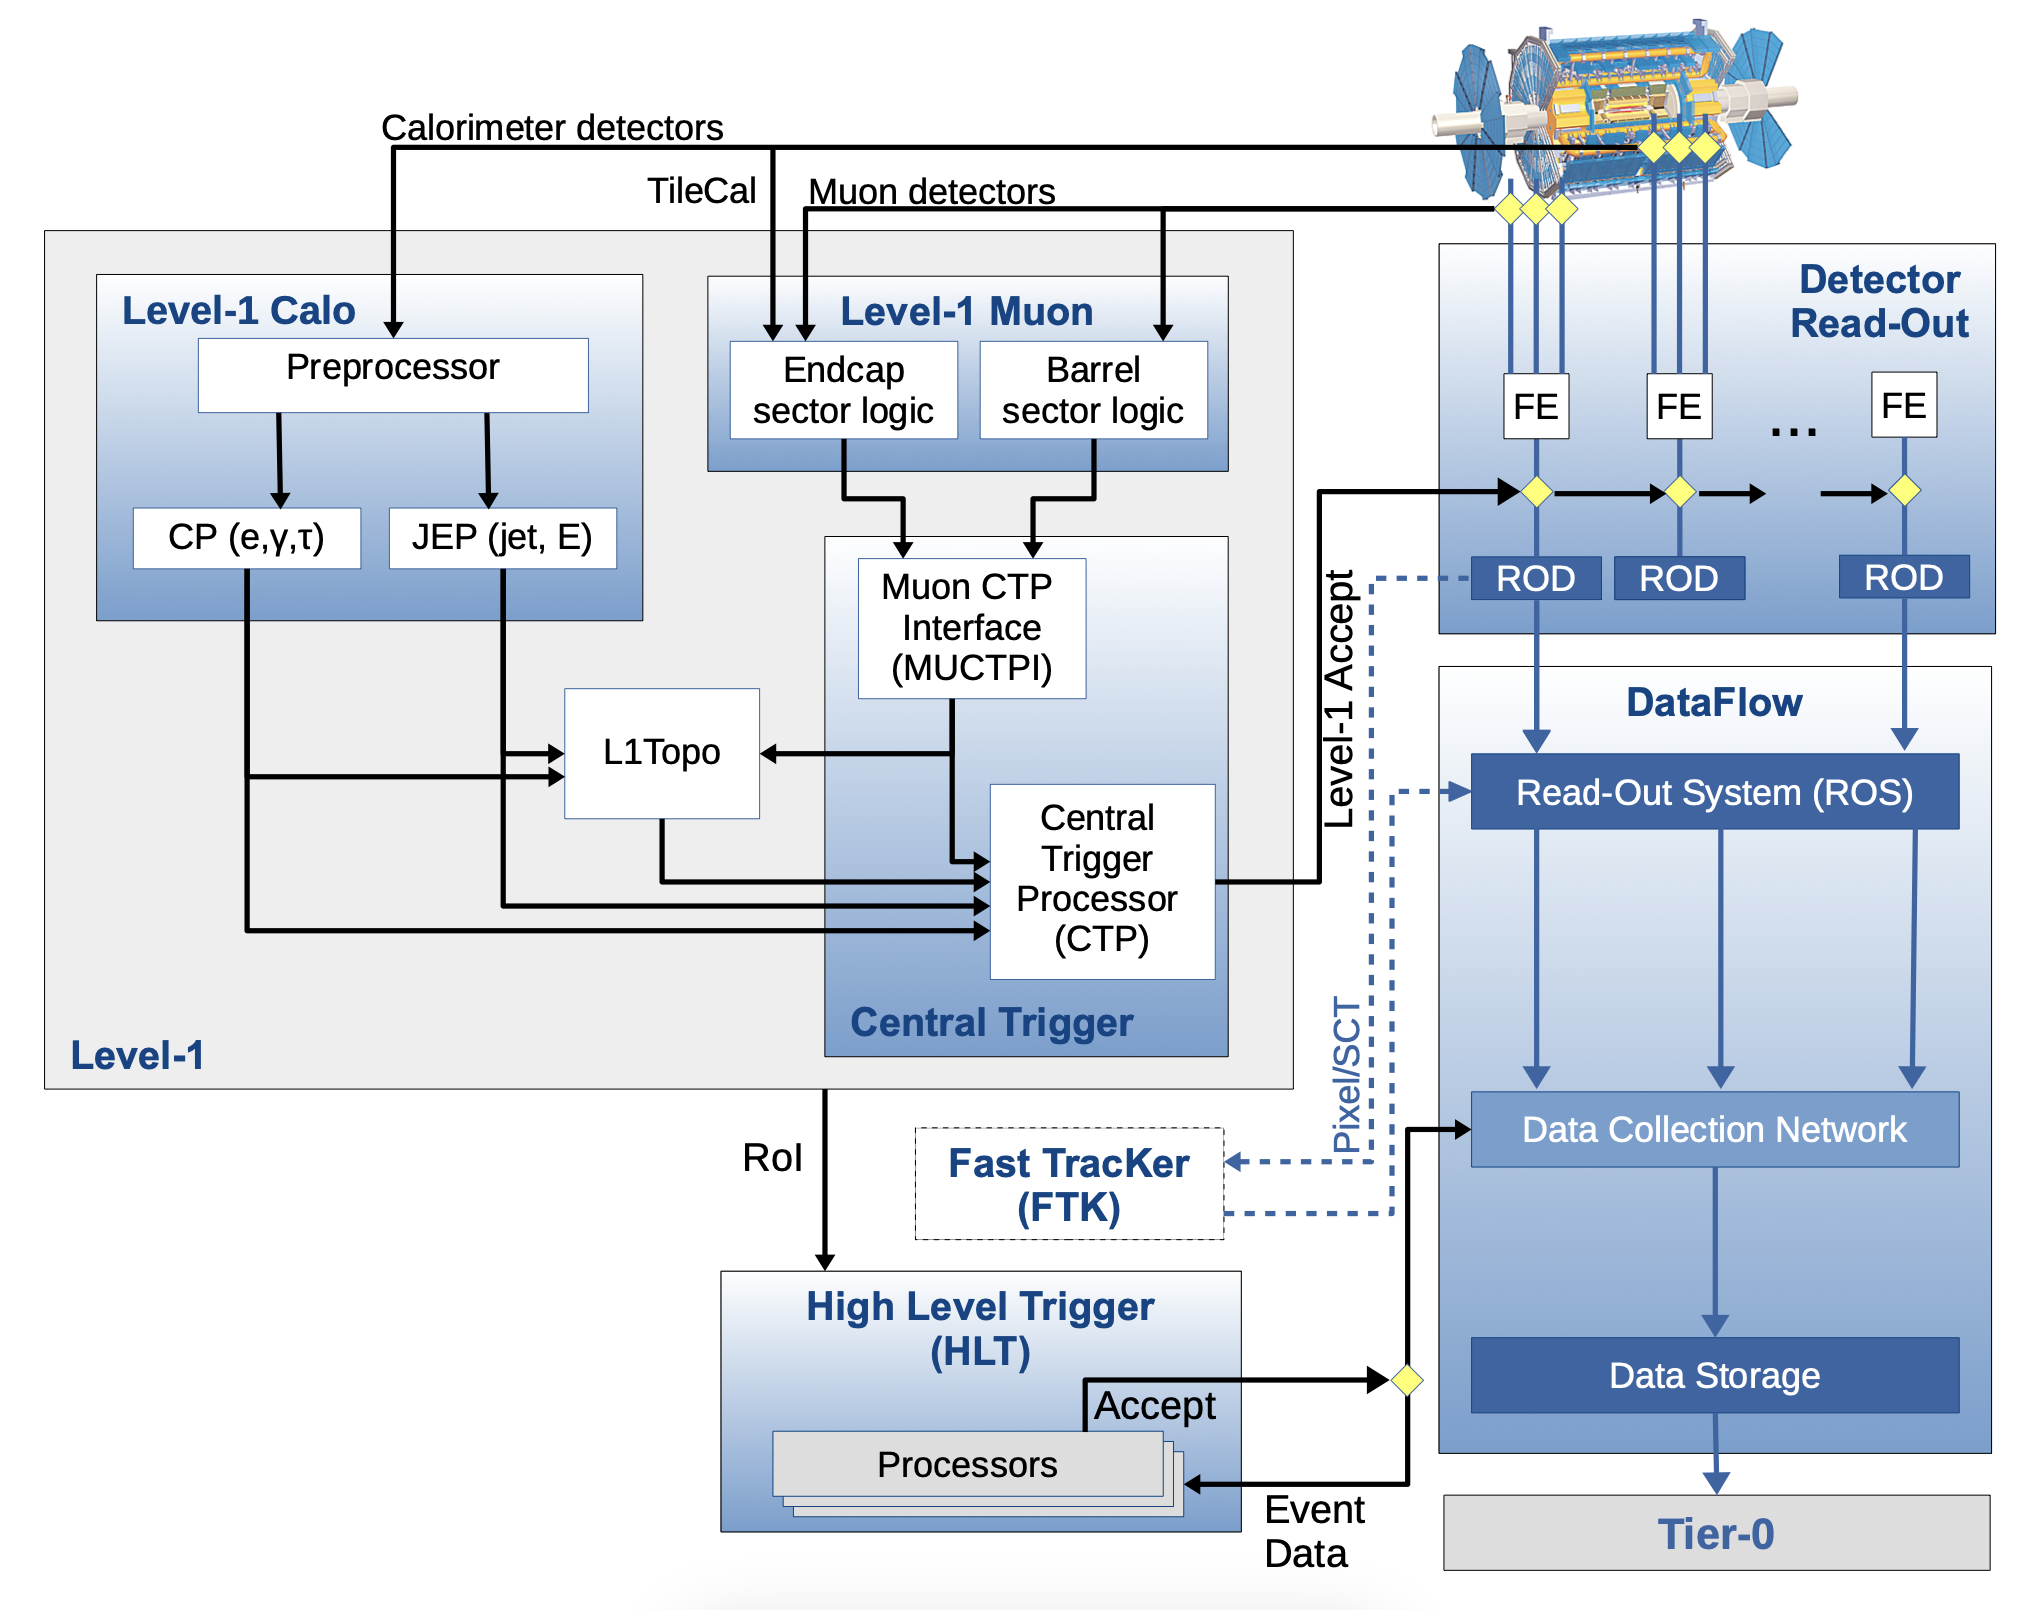
\includegraphics[width=0.99\textwidth]{images/2-LHC-ATLAS/trigger-run-2.png}
    \caption{Schematic layout of the ATLAS Trigger and Data Acquisition system in Run-2, showing the components relevant for triggering as well as the detector read-out and data flow \cite{collaboration_2020}.}
    \label{fig:trigger-run-2-setup}
\end{figure}


%-------------------------------------------
%	Chapter 2: Inner Detector Trigger
%-------------------------------------------
\subsubsection{The Inner Detector Trigger}

The ability of the ATLAS trigger system to process information from the ID to reconstruct particle trajectories is an essential requirement for the efficient triggering of physics objects. The ID trigger must therefore be able to reconstruct tracks with high efficiency across the entire range of possible physics signatures, as well as handle the input rate of the HLT. This challenge is exacerbated by the very high track and hit multiplicities in the ID that arise from the large pile-up. 

The ID trigger is designed to perform fast online track and vertex reconstruction using measurements from the ID. For Run 2, the ID trigger tracking is performed in two steps; the first algorithm handles trigger-specific pattern recognition and seeded track finding to generate medium quality tracks as quickly as possible. This is collectively known as the \textit{Fast Track Finder} (FTF) algorithm \cite{Penc:2104217, Grandi:2624768}. This step is unique to the trigger and is optimized for speed and efficiency with respect to the offline pattern recognition. Optionally, events may be discarded using this information in order to avoid unnecessary downstream processing. This step is followed by the \textit{Precision Tracking} (PT), which relies heavily on offline tracking algorithms \cite{T_Cornelissen_2008} seeded by the spacepoints of the FTF tracks, improving the track purity and resolution of the tracks by applying tighter requirements and by running the so-called \textit{ambiguity removal} tool (see Section \ref{chapter-3-ambiguity-resolution} for further details). 



%-------------------------------------------
%	Chapter 2: Motivation for Hi-Lumi LHC
%-------------------------------------------
\newpage
\section{Motivation for the HL-LHC}
\label{hi-lumi}

% - the physics motivation to increase the luminosity - brief 

% intro
With the accumulated data so far, the identity of the Higgs boson is consistent with SM predictions and all measurements are confined to the couplings of the Higgs to SM particles, which are proportional to the particles’ masses. However, higher-precision measurements of these couplings could illuminate any potential discrepancies from prediction.

% hl-lhc main summary 
The HL-LHC is an upgrade of the \ac{LHC} to extend its physics reach, particularly in terms of precision and reliability in measurements in the Higgs sector, by increasing the data collected by an order of magnitude. This will be achieved by increasing the LHC instantaneous luminosity by a factor of up to five compared to the nominal. This will enable the detector's discovery potential and exploration potential to significantly improve. Initially, the luminosity will be increased to $5 \times 10^{34}  \text{ cm}^{−2}\text{s}^{−1}$, and subsequently up to $7.5 \times 10^{34}  \text{ cm}^{−2}\text{s}^{−1}$ by the mid-2030s. To be able to reach the physics goals set for the HL-LHC, both, the ATLAS and CMS detectors have to be upgraded in order to maintain or improve their performance and physics acceptance, as well as accommodate the higher occupancies and data rates expected at the HL-LHC. These upgrades encompass various components of the detector system. A few of these upgrades are briefly highlighted in the following. More information on the technological and operational challenges is provided in the HL-LHC Preliminary Design Report in Ref \cite{Apollinari:2116337}

% detector upgrades
\subsection{ATLAS Detector Upgrades}
The current ID in ATLAS has various limitations that hinder its performance as the \ac{LHC} machine is upgraded. Radiation damage and high detector occupancy result in the requirement for a full replacement of the ID after Run-3 with the new ITk \cite{pileup,itk-strip}. One significant change in the detector layout is that the ITk will consist only of high granularity silicon detectors, replacing the TRT. This will extend to a 1 m radius, whereas the current SCT outer layer extends only to 60 cm. The acceptance of the detector will be increased such that that the strip detector covers a range of $ \lvert \eta \rvert = 2.7$ with the pixel detector extending the range to $ \lvert \eta \rvert = 4.0$. The improved radiation hardness is designed to cope with greater fluence values in the harsh conditions expected at the HL-LHC. In addition, the ITk material is designed to minimize the effects of multiple scattering and energy losses before particles reach the outer detector components. In addition to this, other parts of the ATLAS detector will also undergo enhancements. The Trigger and Data Acquisition (TDAQ) system will also be extensively redesigned. This redesign aims to provide hardware tracking with full granularity detector data at a selection rate of 1 MHz, while the software-based selection output will be limited to 10 kHz. This upgrade will improve the overall efficiency and performance of the trigger system.


\subsection{Physics Prospects at the HL-LHC}
Since the discovery of the Higgs boson \cite{ATLAS-HIGGS, CMS-HIGGS} in 2012, the study of the Higgs sector has greatly expanded to include many precision measurement analyses, predictions from theory and searches for rare production and decay processes. Despite its phenomenological success, the SM leaves many unanswered questions. Beyond the Standard Model (BSM) theories are devoted to providing answers. 

% higgs self coupling and HH -> 4b
One important question to answer is whether the observed Higgs boson is that predicted from the SM electroweak symmetry breaking mechanism \cite{ewsb} or if it is, in fact, the first signal in some BSM physics. With the accumulated data so far, the identity of the Higgs boson is consistent with SM predictions, but higher-precision measurements could illuminate any potential discrepancies from prediction. While many properties of the Higgs boson can be studied with the current LHC dataset, other properties, such as the Higgs self-coupling cannot be extracted from the existing dataset. Even with the large dataset expected at the HL-LHC, measurements of the Higgs self-coupling are expected to be extremely challenging. The trilinear self-coupling could be a promising window into new physics, which requires the study of the Higgs boson pair productions with a range of decay channels. The $HH \rightarrow b\bar{b}b\bar{b}$ has the largest branching ratio of 33.7\% and is one of the most interesting di-Higgs decays. The pair of $b$-jets from both associated Higgs decays will be closely associated in angle and can therefore be looked into reconstructing the two Higgs as two boosted dijets per event. It is expected that with the combined ATLAS and CMS data, the HL-LHC will only achieve a 4$\sigma$ sensitivity to the di-Higgs signal.


% super symmetry and dark matter
The physics programme offered by the HL-LHC is vast \cite{big-report}. There are many theoretical particles predicted by various BSM scenarios that can also be searched for in the HL-LHC. In general, precision measurements of the Higgs sector provide indirect probes into theoretical particles predicted by BSM scenarios that can also be searched for at higher energy scales. One set of such scenarios falls under the title of Super-Symmetry \cite{supersym}, which predicts super-partners belonging to every fermion and every boson. Direct dark matter searches can also be probed at higher mass scales. The ATLAS and CMS experiments have adopted a set of simplified models which introduce two new particles, a dark matter particle and a mediator, and whose interaction strengths are set by the couplings of the mediator. The HL-LHC phase may allow the experiments to reach these lower couplings and hence probe the hypothetical proposed candidate for dark matter; Weakly Interacting Massive Particles (WIMPs). Additionally, BSM physics can be further probed through rare \textit{b} and \textit{c} hadron decays that may be measured using the increased integrated luminosity \cite{wg-bsm}, and new detector upgrades will facilitate searches for other long-lived exotic particles.


% From a physics point of view why are we upgrading the detector and it stechnologies to higher luminosity?
% pushing the boundaries of what to discover in the hopes of discovering new particles and trying to answer the unanswered questions, physics case for HL-LHC, a comparison on the state of the field now, to where we are going

% https://iopscience.iop.org/article/10.1088/1742-6596/1271/1/012004/pdf


% Close
There are several other theories not mentioned here. Many models are already strongly constrained by existing observations and predict new particles which should be observable at the energy range of the LHC. The LHC experiments will therefore be able to give hints at which theories and models need further attention and will also exclude some models. The HL-LHC programme would deliver a significant potential for new physics discoveries and incredibly high-precision SM measurements. However, the promising plan for the future is accompanied by many technical challenges that each of the experiments face. The increased luminosity results in greater pile-up, which results in drastically higher detector occupancy and radiation levels. In the case of ATLAS, Figure \ref{fig:pileup-walltime} shows the projected evolution of compute usage from 2020 until 2036 under different R\&D scenarios. The expected pile-up levels during the HL-LHC are around $\langle \mu \rangle$ = 200, demonstrating the need for upgrades to both the detector and algorithmic designs.

\begin{figure}[!htbp]
  \centering
  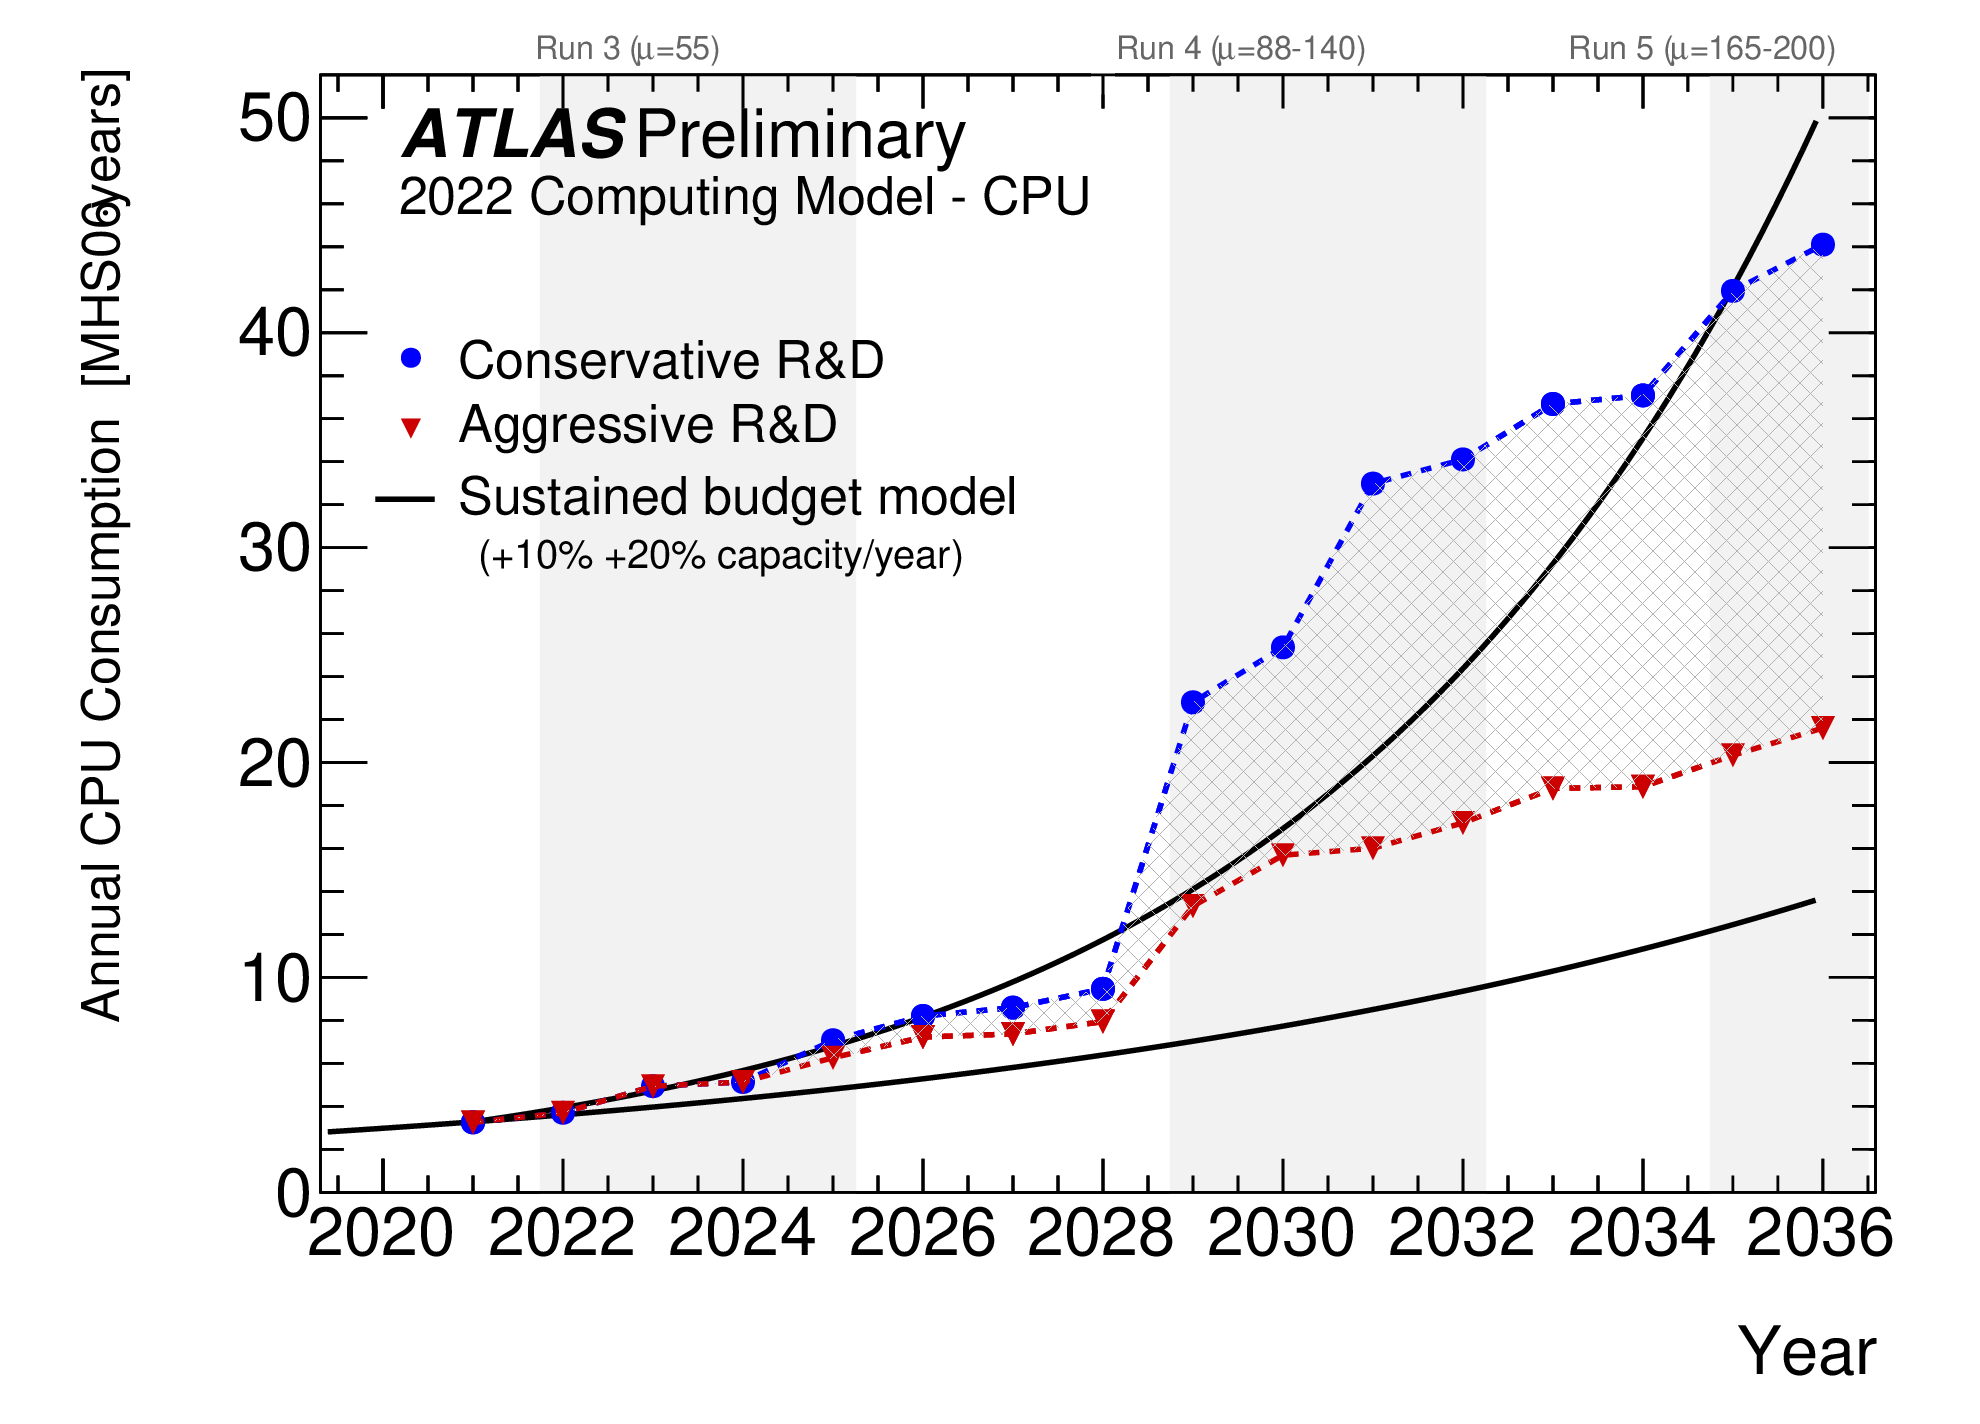
\includegraphics[width=0.8\textwidth]{images/2-LHC-ATLAS/computing-model.png}
  \caption{
    Projected evolution of compute usage under the conservative (blue) and aggressive (red) R\&D scenarios. The darker shading between the red and blue lines illustrates the range of resource consumption if the aggressive scenario is only partially achieved. The black lines indicate the impact of sustained year-on-year budget increases and improvements in new hardware, that together amount to a capacity increase of 10\% (lower line) and 20\% (upper line). The vertical shaded bands indicate periods during which ATLAS will be taking data \cite{Collaboration:2802918}.
  }
  \label{fig:pileup-walltime}
\end{figure}

%In the case of ATLAS, Figure \ref{fig:pileup-walltime} shows how the reconstruction time per event increases with pile-up. The increase in time is exponential, and the expected pile-up levels during the HL-LHC are around $\langle \mu \rangle$ = 200, demonstrating the need for upgrades to both the detector and algorithmic designs in ATLAS.

%\begin{figure}[!htbp]
%  \centering
%  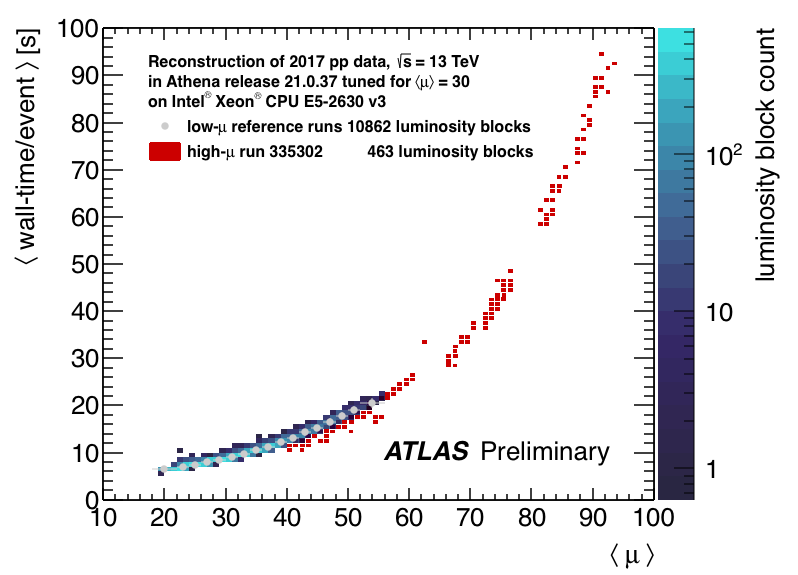
\includegraphics[width=0.8\textwidth]{images/2-LHC-ATLAS/pileup-walltime.png}
%  \caption{
%    The dependency of reconstruction wall time per event on pileup. The luminosity block count represents short intervals of data taking, in which the instantaneous luminosity is estimated, and from this the integrated luminosity derived \cite{pileup}.
%  }
%  \label{fig:pileup-walltime}
%\end{figure}